\labeledsection{Artificial Neural Networks}{sec:ann}
\anondefinition{
An \defemph{Artificial Neural Network (ANN)} is a \linkterm{directed graph}{directed_graph} such that every \linkterm{edge}{undirected_graph} $a_i \to a_j$ is associated with a \defemph{weight} $w_{i,j} \in \mathbb{R}$, and each \linkterm{node}{undirected_graph} $a_j$ with \linkterm{parents}{tree} $a_1, \cdots, a_n$ is associated with a \linkterm{function}{function} $f(w_{1, j}, \cdots w_{n, j}, x_1, \cdots x_n) \in \mathbb{R}$. We call the output of a \linkterm{node}{undirected_graph}'s \linkterm{function}{function} its \defemph{activation}, the matrix $w_{i,j}$ the \defemph{weight matrix}, the \linkterm{nodes}{undirected_graph} \defemph{units} and the \linkterm{edges}{undirected_graph} \defemph{links}
}{ann}

\anondefinition{
A \defemph{McCulloch-Pitts Unit} first computes a weighted sum of all inputs and then applies an \linkterm{activation function}{ann} $g$ to it.
}{mcculloch_pitts}

\anondefinition{
Given a \linkterm{McCulloch-Pitts Unit}{mcculloch_pitts} with an \linkterm{activation function}{ann} $g$. If $g$ is a \linkterm{threshold function}{step_function}, we call the \linkterm{McCulloch-Pitts Unit}{mcculloch_pitts} a \defemph{perceptron unit}, if $g$ is a \linkterm{logistic function}{sigmoid_function}, a \defemph{sigmoid perceptron unit}. 
}{perceptron_sigmoid_unit}

\anondefinition{
A \defemph{McCulloch-Pitts Network} is an \linkterm{Artificial Neural Network}{ann} with \linkterm{McCulloch-Pitts units}{mcculloch_pitts}
}{mcculloch_pitts_network}

\commandnote{
A \linkterm{McCulloch-Pitts Unit}{mcculloch_pitts} computes a linear pre-activation (for example $\mathbf{w}^T\mathbf{x}$). If its activation $g$ is the \linkterm{Heaviside step function}{step_function} the unit implements the \linkterm{Perceptron}{perceptron_hypothesis} — a hard linear classifier trained with the \linkterm{Perceptron Learning Rule}{perceptron_learning_rule}. If $g$ is the \linkterm{logistic function}{sigmoid_function} the unit computes $\sigma(\mathbf{w}^T\mathbf{x})$ and produces a smooth, probability-like score; optimized via gradient-based methods this is the \linkterm{Logistic Regression}{logistic_regression_hypothesis} described in \Secref{sec:regression}. Thus the same McCulloch-Pitts structure with different choices of $g$ connects the perceptron and logistic perspectives: the step activation gives a deterministic decision, while the sigmoid gives a smooth probabilistic output whose $0.5$ threshold recovers the same \linkterm{decision boundary}{decision_boundary} ($\mathbf{w}^T\mathbf{x}=0$).
}

\Example{
We can represent the \texttt{AND} Boolean function as a \linkterm{McCulloch-Pitts Unit}{mcculloch_pitts} with \linkterm{activation function}{ann} $g(r) = 1$ iff $r > 0$, else $0$ (\linkterm{threshold function}{step_function}).

Identify $\texttt{T}=1$ and $\texttt{F}=0$. For inputs $(x_1, x_2) \in \cartprod{\{0,1\}, \{0,1\}}$, choose $x_0=1$ as the dummy input, $w_0=-1$, and $w_1=w_2=1$. Then the weighted sum is
\[
r = w_0x_0 + w_1x_1 + w_2x_2 = -1 + x_1 + x_2.
\]
Now evaluate all four cases:
\[
\begin{array}{c|c|c|c}
x_1 & x_2 & r = -1 + x_1 + x_2 & g(r) \\
\hline
0 & 0 & -1 & 0 \\
0 & 1 & 0 & 0 \\
1 & 0 & 0 & 0 \\
1 & 1 & 1 & 1
\end{array}
\]
So the unit outputs $1$ exactly when both inputs are $1$, which is precisely the \texttt{AND} function.
}{}

\Example{
We can represent the \texttt{OR} Boolean function with the same \linkterm{McCulloch-Pitts Unit}{mcculloch_pitts} setup, again using \linkterm{activation function}{ann} $g(r) = 1$ iff $r > 0$, else $0$ (\linkterm{threshold function}{step_function}).

Identify $\texttt{T}=1$ and $\texttt{F}=0$. For inputs $(x_1, x_2) \in \cartprod{\{0,1\}, \{0,1\}}$, keep $x_0=1$ and $w_1=w_2=1$, but change the bias weight to $w_0=-0.5$. Then the weighted sum is
\[
r = w_0x_0 + w_1x_1 + w_2x_2 = -0.5 + x_1 + x_2.
\]
Now evaluate all four cases:
\[
\begin{array}{c|c|c|c}
x_1 & x_2 & r = -0.5 + x_1 + x_2 & g(r) \\
\hline

0 & 0 & -0.5 & 0 \\
0 & 1 & 0.5 & 1 \\
1 & 0 & 0.5 & 1 \\
1 & 1 & 1.5 & 1
\end{array}
\]
So the unit outputs $1$ whenever at least one input is $1$, which is precisely the \texttt{OR} function.
}{}

\Example{
We can represent the \texttt{NOT} Boolean function with a single-input \linkterm{McCulloch-Pitts Unit}{mcculloch_pitts}, still using \linkterm{activation function}{ann} $g(r) = 1$ iff $r > 0$, else $0$ (\linkterm{threshold function}{step_function}).

Identify $\texttt{T}=1$ and $\texttt{F}=0$. For input $x_1 \in \{0,1\}$, keep $x_0=1$, choose $w_0=0.5$, and choose $w_1=-1$. Then the weighted sum is
\[
r = w_0x_0 + w_1x_1 = 0.5 - x_1.
\]
Now evaluate both cases:
\[
\begin{array}{c|c|c}
x_1 & r = 0.5 - x_1 & g(r) \\
\hline
0 & 0.5 & 1 \\
1 & -0.5 & 0
\end{array}
\]
So the unit outputs $1$ exactly when the input is $0$, which is precisely the \texttt{NOT} function.
}{}

\begin{figure}[H]
    \centering
    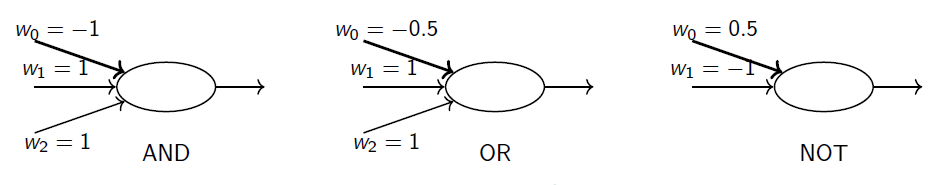
\includegraphics[width=0.5\linewidth]{images/and_or_not.png}
\end{figure}

\observationbox{
By stacking \linkterm{McCulloch-Pitts units}{mcculloch_pitts} into a \linkterm{McCulloch-Pitts Network}{mcculloch_pitts_network}, we can combine simple thresholded units into a larger computation. In particular, since any Boolean function can be written using combinations of \texttt{AND}, \texttt{OR}, and \texttt{NOT}, a finite network of \linkterm{threshold function}{step_function} units can implement any Boolean function on finitely many binary inputs.
}


\Theorem{
Every Boolean function on finitely many binary inputs can be implemented as a \linkterm{McCulloch-Pitts Network}{mcculloch_pitts_network}
}{}

\Example{
The \texttt{XOR} function
\[
x_1 \oplus x_2 = (x_1 \lor x_2) \land \neg (x_1 \land x_2)
\]
can be built from a small \linkterm{McCulloch-Pitts Network}{mcculloch_pitts_network}:

\begin{figure}[H]
    \centering
    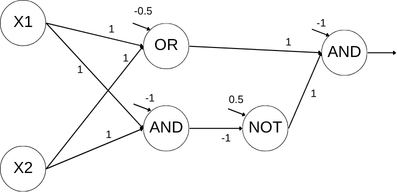
\includegraphics[width=0.3\linewidth]{images/xor_unitsnetwork.png}
\end{figure}
}{}


\anondefinition{
A \linkterm{Neural Network}{ann} is called a \defemph{Feed-Forward Neural Network}, if it is \linkterm{acyclic}{cyclic_graphs}
}{ffnn}

\anondefinition{
A \defemph{perceptron network} is a \linkterm{Feed-Forward Neural Network}{ffnn} of \linkterm{perceptron units}{mcculloch_pitts} (\linkterm{threshold}{step_function}-\linkterm{activated}{ann} \linkterm{McCulloch‑Pitts units}{mcculloch_pitts} ).
}{perceptron_network}

\anondefinition{
\linkterm{Feed-Forward Neural Networks}{ffnn} are usually organized in \defemph{layers}: a \defemph{$n$ layer network} has a partition $\set{L_0, \cdots, L_n}$ of the \linkterm{nodes}{undirected_graph}, such that \linkterm{edges}{undirected_graph} only connect \linkterm{nodes}{undirected_graph} from subsequent \defemph{layer}. $L_0$ is called the \defemph{input layer} and its members \defemph{input units}, and $L_n$ the \defemph{output layer} and its members \defemph{output units}. Any \defemph{unit} that is not in the \defemph{input layer} or the \defemph{output layer} is called \defemph{hidden}
}{layers_neural_nets}

\anondefinition{
A single-\linkterm{layer}{layers_neural_nets} \linkterm{perceptron network}{perceptron_network} is called a \defemph{perceptron}
}{perceptron_nn}

\Example{
\begin{figure}[H]
    \centering
    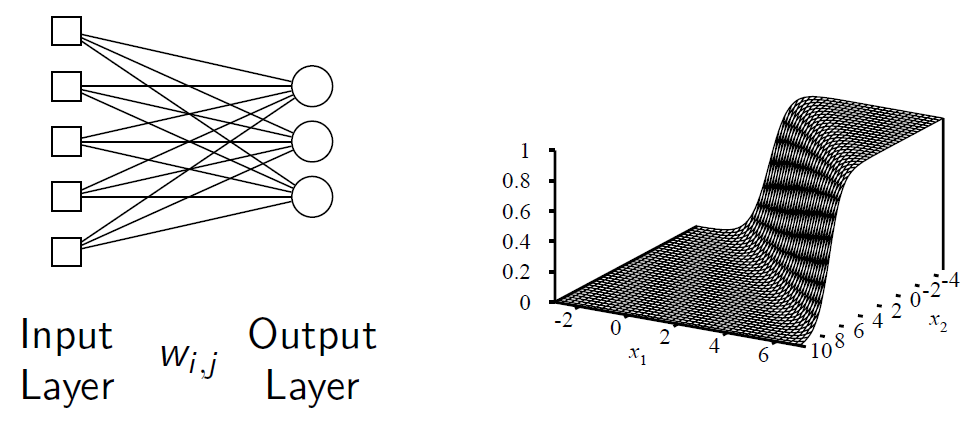
\includegraphics[width=0.3\linewidth]{images/perceptron.png}
\end{figure}
}{}

\titledbox{Expressivity of Perceptrons}{
\linkterm{Perceptrons}{perceptron_nn} can represent \texttt{AND}, \texttt{OR}, \texttt{NOT}, etc. but not \texttt{XOR}. They represent \linkterm{linear separator}{decision_boundary} in input space
}

\begin{figure}[H]
    \centering
    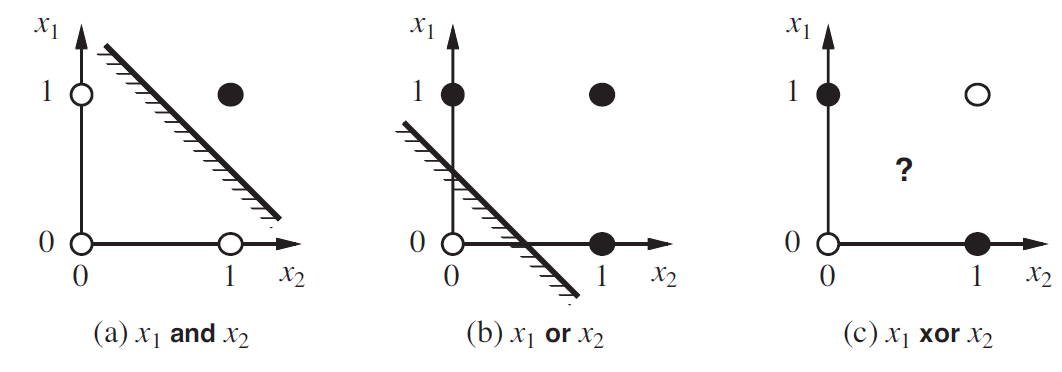
\includegraphics[width=0.5\linewidth]{images/no_xor.png}
\end{figure}

\questionbox{
How \linkterm{perceptrons}{perceptron_nn} learn? (how we update the weights?)
}

\answerbox{
Recall the \linkterm{perceptron learning rule}{perceptron_learning_rule} for \linkterm{multivariate linear regression}{multivariate_linear_regression}.

Single-output (vector form). Let $\mathbf{x}^{(i)}\in\mathbb{R}^{n+1}$ include the bias coordinate $x_0=1$, label $y^{(i)}\in\{0,1\}$, and prediction $\hat{y}^{(i)}=\mathcal{T}(\mathbf{w}^T\mathbf{x}^{(i)})$. The online perceptron update is:
\[
\mathbf{w}^{(t+1)} := \mathbf{w}^{(t)} + \alpha\big(y^{(i)} - \hat{y}^{(i)}\big)\,\mathbf{x}^{(i)}.
\]

Multi-output (single-layer) perceptron. For $K$ output units use a weight matrix $W = (w_{j,k})$, where $j$ indexes the input node and $k$ indexes the output unit. In other words, $w_{j,k}$ is the weight on the edge from the $j$th input unit to the $k$th output unit, and for a fixed $k$ the vector $\mathbf{w}_k = (w_{0,k}, w_{1,k}, \cdots, w_{n,k})^T$ collects all weights feeding into output unit $k$. For each output unit $k$:
\[
\mathbf{w}_k^{(t+1)} := \mathbf{w}_k^{(t)} + \alpha\big(y_k^{(i)} - \hat{y}_k^{(i)}\big)\,\mathbf{x}^{(i)},
\]
or coordinate-wise
\[
w_{j,k}^{(t+1)} := w_{j,k}^{(t)} + \alpha\big(y_k^{(i)} - \hat{y}_k^{(i)}\big) x_j^{(i)}.
\]

\begin{figure}[H]
    \centering
    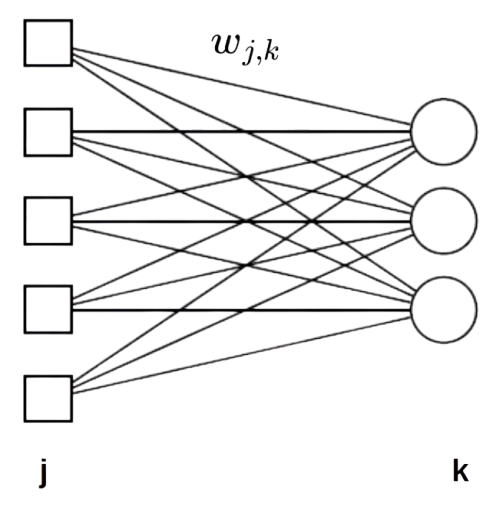
\includegraphics[width=0.2\linewidth]{images/perceptron_update.png}
\end{figure}
}

\questionbox{
What changes when the activation function is smooth and differentiable instead of a threshold?
}

\answerbox{
If a network has multiple outputs, each output unit $k$ computes its own activation using its specific weight vector $\mathbf{w}_k$:
\[
h_{\mathbf{w}_k}(\mathbf{x}^{(i)}) := g\big(\mathbf{w}_k^T\mathbf{x}^{(i)}\big).
\]
Where $g$ is differentiable, we minimize the total squared error loss over all $K$ output units, $L = \frac{1}{2}\sum_{m=1}^K \big(y_m^{(i)} - h_{\mathbf{w}_m}(\mathbf{x}^{(i)})\big)^2$, by gradient descent.

For a single coordinate $w_{j,k}$ feeding into output unit $k$, the partial derivative isolates to that specific unit via the chain rule:
\[
\frac{\partial L}{\partial w_{j,k}}
=
\frac{\partial L}{\partial h_{\mathbf{w}_k}(\mathbf{x}^{(i)})}
\cdot g'\big(\mathbf{w}_k^T\mathbf{x}^{(i)}\big)
\cdot x_j^{(i)}.
\]

The resulting online gradient descent update rule becomes:
\[
w_{j,k}^{(t+1)} := w_{j,k}^{(t)} + \alpha\big(y_k^{(i)} - h_{\mathbf{w}_k}(\mathbf{x}^{(i)}\big)\big)\, g'\big(\mathbf{w}_k^T\mathbf{x}^{(i)}\big)\, x_j^{(i)}.
\]
So the only extra factor compared to the multi-output perceptron update is the derivative of the activation function, $g'$, evaluated at the weighted sum for unit $k$.
}

\anondefinition{
In \defemph{Multi-Layer Perceptrons (MLPs)}, \linkterm{layers}{layers_neural_nets} are usually fully connected; number of \linkterm{hidden units}{layers_neural_nets} typically chosen by hand
\begin{figure}[H]
    \centering
    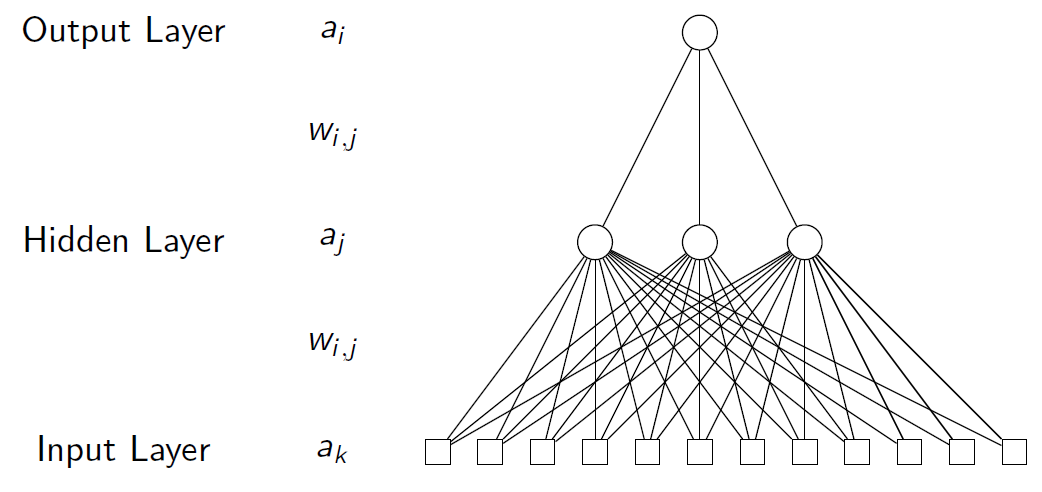
\includegraphics[width=0.5\linewidth]{images/mlp.png}
\end{figure}
}{mlps}

\observationbox{
What we did in the \texttt{XOR} example is actually a \linkterm{MLPs}{mlps}
}

\observationbox{
It allowed us to express a non-linear function (the \texttt{XOR} function)
}

\ideabox{
We can train \linkterm{MLPs}{mlps} on non-linear data! The \linkterm{output layer}{layers_neural_nets} can be viewed as a differentiable classifier whose input is the activation vector of the last \linkterm{hidden layer}{layers_neural_nets} $\leadsto$ we can use gradient descent to update the weights of the \linkterm{output layer}{layers_neural_nets} directly based on the true targets. 
}

\problembox{
What about the \linkterm{hidden layers}{layers_neural_nets}? We do not have some notion of \textit{"lost / error"} there. How to update the weights ?
}

\ideabox{
The hidden node $j$ is \textit{"responsible"} for some fraction of the error proportional to the weight $w_{j,k}$
}

\commandnote{
For the \linkterm{output layer}{layers_neural_nets}, the error is clear because we can compare the prediction directly against the true label $y_k^{(i)}$. For a \linkterm{hidden layer}{layers_neural_nets}, we do not have target labels. 
}

\ideabox{
every \linkterm{hidden unit}{layers_neural_nets} $j$ contributes to the inputs of the next layer's units. Therefore, the total error observed at the \linkterm{output layer}{layers_neural_nets} is an accumulation of the errors \textbf{propagated forward} from the \linkterm{hidden layers}{layers_neural_nets}. 
}

\questionbox{
Can we \textbf{Back Propagate} the error?
}

\answerbox{
Yes, this is where the Backpropagation algorithm comes to the rescue.
}
\titledbox{Backpropagation Intuition}{
The core intuition of the \textbf{Backpropagation algorithm} is to take the error from the output layer and pass it \textbf{backward} through the network matrix, reversing the direction of the forward pass. A hidden node $j$ is penalized based on how much it contributed to the error of the units in the subsequent layer, scaled by the strength of the connecting weight $w_{j,k}$.
}

\redbox{
To achieve that, we need the \linkterm{activation function}{ann} of all units to be differentiable, hence we can no longer use the \linkterm{threshold function}{step_function}. Instead, we switch to a smooth, differentiable activation function, such as the \linkterm{logistic function}{sigmoid_function} $\sigma(r) = \frac{1}{1 + e^{-r}}$.
}

\titledbox{Remember}{
We update the weights using online gradient descent:
\[
w_{j,k} \leftarrow w_{j,k} + \alpha\big(y_k^{(i)} - h_{\mathbf{w}_k}(\mathbf{x}^{(i)})\big)\, g'\big(\mathbf{w}_k^T\mathbf{x}^{(i)}\big)\, x_j^{(i)}.
\]
}

\observationbox{
The term $\big(y_k^{(i)} - h_{\mathbf{w}_k}(\mathbf{x}^{(i)})\big)\, g'\big(\mathbf{w}_k^T\mathbf{x}^{(i)}\big)$ represents the error at \linkterm{output unit}{layers_neural_nets} $k$. We refer to that as $\delta_k$.
}

\titledbox{Justification}{
To understand the exact origin of the output error signal $\delta_k$, we derive the weight update directly from the foundational principles of gradient descent, parsing the network mechanics from the parameters upward to the loss function.
}

\paragraph{Step 1:}
Our objective is to minimize the total squared error loss $L$ across all $K$ output units for a single training instance $\mathbf{x}^{(i)}$:
\[
L = \frac{1}{2}\sum_{m=1}^K \big(y_m^{(i)} - h_{\mathbf{w}_m}(\mathbf{x}^{(i)})\big)^2
\]
To optimize a specific weight $w_{j,k}$ connecting an incoming unit $j$ to an output unit $k$, the standard online gradient descent update rule dictates that we move in the negative direction of the gradient:
\[
w_{j,k} \leftarrow w_{j,k} - \alpha \frac{\partial L}{\partial w_{j,k}}
\]

\paragraph{Step 2: Chain Rule}
Because the weight $w_{j,k}$ does not influence the loss directly, its impact passes through the net input (pre-activation sum) of output unit $k$, which we define as $r_k^{(i)} = \mathbf{w}_k^T\mathbf{x}^{(i)} = \sum_{m} w_{m,k} x_m^{(i)}$. 



By applying the calculus chain rule, we can break down our target partial derivative into two operational components:
\[
\frac{\partial L}{\partial w_{j,k}} = \frac{\partial L}{\partial r_k^{(i)}} \cdot \frac{\partial r_k^{(i)}}{\partial w_{j,k}}
\]

\paragraph{Step 3:}
The second term represents how changing the weight alters the linear combination passing into unit $k$. Since $r_k^{(i)} = w_{0,k}x_0^{(i)} + \cdots + w_{j,k}x_j^{(i)} + \cdots + w_{n,k}x_n^{(i)}$, differentiating with respect to $w_{j,k}$ treats all other components as constants and isolates the value of the incoming activation signal:
\[
\frac{\partial r_k^{(i)}}{\partial w_{j,k}} = x_j^{(i)}
\]
Substituting this back into our chain rule equation yields:
\[
\frac{\partial L}{\partial w_{j,k}} = \frac{\partial L}{\partial r_k^{(i)}} \cdot x_j^{(i)}
\]

\paragraph{Step 4:}
The remaining partial derivative, $\frac{\partial L}{\partial r_k^{(i)}}$, measures how sensitive the total network loss is to changes in the pre-activation state of output unit $k$. Since the final output activation is determined by our smooth function $h_{\mathbf{w}_k}(\mathbf{x}^{(i)}) = g(r_k^{(i)})$, we apply the chain rule one final time:
\[
\frac{\partial L}{\partial r_k^{(i)}} = \frac{\partial L}{\partial h_{\mathbf{w}_k}(\mathbf{x}^{(i)})} \cdot \frac{\partial h_{\mathbf{w}_k}(\mathbf{x}^{(i)})}{\partial r_k^{(i)}}
\]

We evaluate these two simple derivatives independently:
\begin{enumerate}
    \item \textbf{Loss with respect to Activation:} When differentiating $\frac{1}{2}\sum_{m=1}^K \big(y_m^{(i)} - h_{\mathbf{w}_m}(\mathbf{x}^{(i)})\big)^2$ with respect to the specific output unit activation $h_{\mathbf{w}_k}$, all terms where $m \neq k$ become zero, leaving:
    \[
    \frac{\partial L}{\partial h_{\mathbf{w}_k}(\mathbf{x}^{(i)})} = 2 \cdot \frac{1}{2} \big(y_k^{(i)} - h_{\mathbf{w}_k}(\mathbf{x}^{(i)})\big)^{2-1} \cdot (-1) = -\big(y_k^{(i)} - h_{\mathbf{w}_k}(\mathbf{x}^{(i)})\big)
    \]
    \item \textbf{Activation with respect to Pre-Activation:} Differentiating the activation function with respect to its internal net input simply leaves the local derivative:
    \[
    \frac{\partial h_{\mathbf{w}_k}(\mathbf{x}^{(i)})}{\partial r_k^{(i)}} = g'\big(r_k^{(i)}\big) = g'\big(\mathbf{w}_k^T\mathbf{x}^{(i)}\big)
    \]
\end{enumerate}

Combining these two evaluations back together gives us:
\[
\frac{\partial L}{\partial r_k^{(i)}} = -\big(y_k^{(i)} - h_{\mathbf{w}_k}(\mathbf{x}^{(i)})\big) \cdot g'\big(\mathbf{w}_k^T\mathbf{x}^{(i)}\big)
\]

\paragraph{Step 5:}
We isolate this internal sensitivity term and define its negative value as the localized error signal, denoted by the shorthand variable $\delta_k$:
\[
\delta_k \equiv -\frac{\partial L}{\partial r_k^{(i)}} = \big(y_k^{(i)} - h_{\mathbf{w}_k}(\mathbf{x}^{(i)})\big)\, g'\big(\mathbf{w}_k^T\mathbf{x}^{(i)}\big)
\]

Reassembling back into the total loss derivative from Step 3:
\[
\frac{\partial L}{\partial w_{j,k}} = -\delta_k x_j^{(i)}
\]

Finally, we substitute this back into our original gradient descent statement from Step 1. The two negative signs cancel out perfectly, yielding our final operational update rule:
\[
w_{j,k} \leftarrow w_{j,k} + \alpha \delta_k x_j^{(i)}
\]


\problembox{
How do we define the error signal $\delta_j$ for a hidden unit $j$ when there is no true target $y_j^{(i)}$ available?
}

\paragraph{Step 1:}
Let $j$ be a node in a hidden layer $L_{n-1}$. Just like we did for the output layer, we define its local error signal $\delta_j$ as the sensitivity of the total loss $L$ with respect to its pre-activation net input $r_j^{(i)}$:
\[
\delta_j \equiv -\frac{\partial L}{\partial r_j^{(i)}}
\]
We expand this using the chain rule. Because the pre-activation $r_j^{(i)}$ directly influences the loss only through its output activation $a_j^{(i)} = g(r_j^{(i)})$, we write:
\[
\delta_j = -\frac{\partial L}{\partial a_j^{(i)}} \cdot \frac{\partial a_j^{(i)}}{\partial r_j^{(i)}}
\]

\paragraph{Step 2:}
The second term is straightforward. Since $a_j^{(i)} = g(r_j^{(i)})$, its partial derivative with respect to its pre-activation is simply the derivative of the activation function:
\[
\frac{\partial a_j^{(i)}}{\partial r_j^{(i)}} = g'\big(r_j^{(i)}\big)
\]
Substituting this back gives:
\[
\delta_j = -\frac{\partial L}{\partial a_j^{(i)}} \cdot g'\big(r_j^{(i)}\big)
\]

\paragraph{Step 3: Backpropagation}
Now we face the core problem: finding $\frac{\partial L}{\partial a_j^{(i)}}$. How does a change in hidden unit $j$'s activation affect the final loss? 

It affects the loss because unit $j$ sends its activation forward to \textbf{every single unit $k$ in the next layer}. Each unit $k$ computes a pre-activation $r_k^{(i)} = \sum_{m} w_{m,k} a_m^{(i)}$, which includes the term $w_{j,k} a_j^{(i)}$. 

Therefore, a change in $a_j^{(i)}$ changes \textbf{all} pre-activations in the subsequent layer. By the multi-variable chain rule, we must sum up the gradients passing through all units $k$ that receive a link from node $j$:
\[
\frac{\partial L}{\partial a_j^{(i)}} = \sum_{k} \frac{\partial L}{\partial r_k^{(i)}} \cdot \frac{\partial r_k^{(i)}}{\partial a_j^{(i)}}
\]



\paragraph{Step 4:}
We can simplify the terms inside this summation easily:
\begin{enumerate}
    \item From our output layer derivation, we already know that $\frac{\partial L}{\partial r_k^{(i)}} = -\delta_k$.
    \item Differentiating the next layer's pre-activation $r_k^{(i)} = \dots + w_{j,k} a_j^{(i)} + \dots$ with respect to $a_j^{(i)}$ isolates the connecting weight parameter:
    \[
    \frac{\partial r_k^{(i)}}{\partial a_j^{(i)}} = w_{j,k}
    \]
\end{enumerate}

Plugging these back into the sum yields:
\[
\frac{\partial L}{\partial a_j^{(i)}} = \sum_{k} (-\delta_k) \cdot w_{j,k} = -\sum_{k} w_{j,k} \delta_k
\]

\paragraph{Step 5:}
Now, we substitute this summation result back into our equation for $\delta_j$ from Step 2. The two negative signs cancel out perfectly, giving us the elegant recurrence relation of backpropagation:
\[
\delta_j = g'\big(r_j^{(i)}\big) \sum_{k} w_{j,k} \delta_k
\]

\observationbox{
This shows that the error signal $\delta_j$ of a hidden unit is simply the derivative of its activation function multiplied by the weighted sum of the error signals $\delta_k$ from the subsequent layer. The error is literally flowing \textbf{backward} through the weights!
}


\titledbox{Summary: The Four Core Equations}{
For any feed-forward neural network using smooth differentiable activation functions, the entire learning workflow per training instance $\mathbf{x}^{(i)}$ can be summarized by four mathematical equations using our established indices $j$ (source hidden unit) and $k$ (destination unit):

\begin{itemize}
    \item Output Error: $\delta_k = \big(y_k^{(i)} - h_{\mathbf{w}_k}(\mathbf{x}^{(i)})\big)\, g'\big(r_k^{(i)}\big)$
    \item Hidden Error: $\delta_j = g'\big(r_j^{(i)}\big) \sum_{k} w_{j,k} \delta_k$
    \item Gradient Calculation: $ \frac{\partial L}{\partial w_{j,k}} = -\delta_k a_j^{(i)}$
    \item Weight Update: $w_{j,k} \leftarrow w_{j,k} + \alpha \delta_k a_j^{(i)}$
\end{itemize}
}

\anondefinition{
The \defemph{Back-Propagation Rule} for \linkterm{hidden nodes}{layers_neural_nets} of a \linkterm{multilayer perceptron}{mlps} is:
\[
\delta_j = g'\big(r_j^{(i)}\big) \sum_{k} w_{j,k} \delta_k
\]
and the update rule for weights in a \linkterm{hidden layer}{layers_neural_nets} is:
\[
w_{j,k} \leftarrow w_{j,k} + \alpha \delta_k a_j^{(i)}
\]
}{backpropagation}

\anondefinition{
The \defemph{Backpropagation Learning Algorithm} is given by the following pseudocode:
\begin{algorithm}[H]
\caption{Stochastic Backpropagation Algorithm}
\label{alg:backprop}
\begin{algorithmic}[1]
\Function{Backpropagation}{examples, $\alpha$}
\State inputs: \textit{examples}, a set of training pairs $(\mathbf{x}^{(i)}, \mathbf{y}^{(i)})$; $\alpha$, the learning rate
\State local variables: network weights $w_{j,k}$ initialized to small random numbers
\Repeat
    \For{each training instance $(\mathbf{x}^{(i)}, \mathbf{y}^{(i)})$ in \textit{examples}}
        \State \textbf{Forward Pass:}
        \State Compute activation values layer-by-layer from input layer $L_0$ to output layer $L_n$
        
        \State \textbf{Backward Pass:}
        \For{each unit $k$ in output layer $L_n$}
            \State $\delta_k \leftarrow \big(y_k^{(i)} - h_{\mathbf{w}_k}(\mathbf{x}^{(i)})\big)\, g'\big(r_k^{(i)}\big)$
        \EndFor
        
        \For{each hidden layer from $L_{n-1}$ down to $L_1$}
            \For{each unit $j$ in current hidden layer}
                \State $\delta_j \leftarrow g'\big(r_j^{(i)}\big) \sum_{k} w_{j,k} \delta_k$
            \EndFor
        \EndFor
        
        \State \textbf{Weight Update Step:}
        \For{each weight $w_{j,k}$ in network}
            \State $w_{j,k} \leftarrow w_{j,k} + \alpha \delta_k a_j^{(i)}$
        \EndFor
    \EndFor
\Until{convergence criteria are satisfied}
\State \Return network weights $w_{j,k}$
\EndFunction
\end{algorithmic}
\end{algorithm}
}{backpropagation_alg}

